\chapter{Results}
We test each of the specified variables over a range of values to examine trends in the reconstruction speed and overall accuracy. Unless otherwise noted, the default values for each simulation are listed in Table \ref{tab:def_vals}. Our error bars represent one standard deviation away from the mean and are calculated under the assumption of Gaussian noise. We assume this to be a good approximation of the true noise distribution based on the central limit theorem of statistics ***(make sure you've explained).\\

\begin{table}[h]
    \centering
    \begin{tabular}{|c|c|c|c|c|c|c|c|}
    \hline
    Variable: & Precision & Total hits & Hits used & P-value & $\eta'$-tolerance & $\sigma_{sp}$ & $a$ \\
    \hline
    Value: & single & 5 & 5 & 0.01 & 1.0 & 1 mm & 0.22 \\
    \hline
    \end{tabular}
    \caption{Caption}
    \label{tab:def_vals}
\end{table}

\section{Power}
To measure the power our hardware uses when running, we use the WITRN U2 USP Power Monitor\cite{WITRN}. Our original estimate for how much power usage would be acceptable aboard a telescope array was about 50 W based on past experience. We tested the Raspberry Pi's power usage and found that it ranged from about 2.52 W when idle to 2.74 W on average after running the program for a few hours. The differential power usage, found by subtracting the idle power from the power running the reconstruction algorithm, was 0.23 W on average. Though our USB monitor did not allow us to calculate its standard deviation, our maximum total and differential powers were 4.82 W and 2.30 W, respectively, which are both an order of magnitude less than our estimated power budget. We expect that the hardware in the telescope design will be similar to the raspberry pi, so it is likely that the true power used will be similar to these values.

\section{Precision}
The precision of our floating point values refers to how many bits we use in calculation. We use single-precision (32-bit) \texttt{float} values and double-precision (64-bit) \texttt{double} values in our calculations, and test them against each other. The results of our test runs are shown in Table \ref{tab:floatvdouble}. We see that we get slightly less accuracy on average when using float values rather than double values, but there is a large overlap in the two margins of error, so this is not a very statistically significant result. However, we also see a large decrease in reconstruction speed when using double values compared to floats. This is an expected result, as basic operations take longer for 64-bit values than for 32-bit values regardless of the hardware. This effect is less pronounced on Cassini as it has an out-of-order processor which can use its idle clock cycles to perform instructions for future use, decreasing the overall runtime. Unfortunately, the raspberry pi is an in-order processor and does not have such capabilities, so it is best that we use single-precision values in our final version of the program to increase the throughput.

\begin{table}[h]
    \centering
    \begin{tabular}{|c|c|c|}
        \hline
        Precision &  Single & Double \\
        \hline
        Accuracy (\%) & 86.12 $\pm$ .12 & 86.15 $\pm$ .10 \\
        \hline
        Throughput ($\gamma/sec$) & \num{5.08 \pm 0.70 e5} & \num{3.85 \pm .51 e5} \\
        \hline
    \end{tabular}
    \caption{Caption}
    \label{tab:floatvdouble}
\end{table}

\section{Parallelism}
We test our algorithms' parallelism on Cassini as it has more cores. This speedup is calculated for both latency and throughput. Latency is defined here as the inverse of the execution speed: $L = \frac{1}{v} = \frac{T}{W}$, where $v$ is the execution speed, $T$ is the program's runtime, and $W$ is the work done by the program. The speedup in latency between programs 1 and 2 is then defined by $S_L = \frac{L_1}{L_2} = \frac{T_1 W_2}{T_2 W_1}$. As the work done by our program is approximately the same each time, this simplifies to $S_L = \frac{T_1}{T_2}$. In this case, $T_1$ is our base runtime, with only one core, while $T_2$ ranges from one to 24, the max number of cores on Cassini. The results are shown in Figure \ref{fig:latency_speedup}.

We define throughput here as the execution rate of a task: $Q = \rho v A = \frac{\rho A}{L}$, where $\rho$ is the number of stages in the pipeline and $A$ is the number of processors available. The latency in throughput is then $S_Q = \frac{Q_2}{Q_1} = \frac{\rho_2 A_2}{\rho_1 A_1} S_L$. Since $\rho$ is the same for each run of the program, $S_Q = \frac{A_2}{A_1} S_L$, which is shown in Figure \ref{fig:through_speedup}. We can see that we have near-linear speedup when the number of cores is small, but still have an overall linear trend at higher numbers of cores. This indicates that our program scales well with increased execution capacity.

\begin{figure}
    \centering
    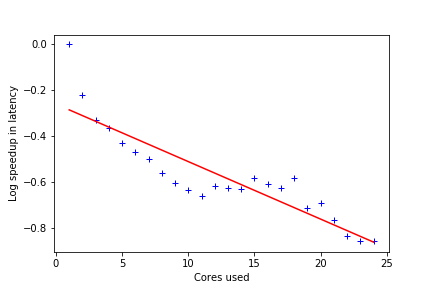
\includegraphics[width=0.7\textwidth]{graphs/Cassini_latency_speedup.png}
    \caption{Speedup of reconstruction algorithm in latency.}
    \label{fig:latency_speedup}
\end{figure}

\begin{figure}
    \centering
    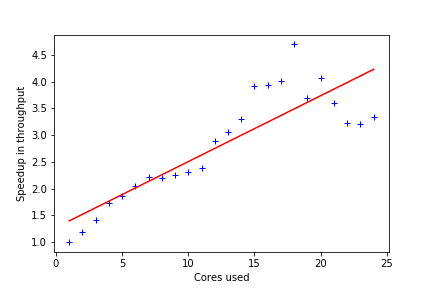
\includegraphics[width=0.7\textwidth]{graphs/Cassini_throughput_speedup.png}
    \caption{Speedup of reconstruction algorithm in throughput.}
    \label{fig:through_speedup}
\end{figure}

%%% Number of hits

\section{Total hits used}
To ensure that our program is behaving the way we want it to, we investigate its behavior using events with various numbers of hits. We can see from Figure \ref{fig:hits_speed} that our throughput decreases exponentially with increasing numbers of simulated hits. While not ideal, this is an improvement on our original estimate of a factorial increase in computation time. Though, theoretically, the worst-case time complexity of our program remains the same as in the iterative version, tree search improves the average-case complexity of our search algorithm and displays improved performance over a large number of simulated photons.

In plotting the accuracy of our program for increasing numbers of hits (Figure \ref{fig:hits_acc}) we find some interesting results. The accuracy peaks at 5 hits simulated. It is unclear from the algorithm exactly why this is, but it is possible that increasing the number of hits past a certain point introduces more error, while having fewer hits to work with does not constrain the problem enough. If a similar trend holds for testing on more accurate simulators, we may consider weighting our angle reconstructions based on these probabilities, using them as a prior when we calculate our final source position from the available angle reconstructions.

- We can see that our throughput appears to go down exponentially as we increase the number of hits for each event. This is an improvement on our original algorithm, which had a complexity of N!. If our only speed improvements were the results of parallelism, we would still expect to see factorial time complexity, but this shows that our tree search algorithm has improved the average-case runtime of our program.

- Though we use $\chi^2$-pruning on our tree search algorithm, we still are performing this operation sequentially within each of our parallel threads. We have not implemented this parallelism yet since we have already reached our current timing goals, but if we ever need to improve the runtime further we could always introduce parallelism into the tree search itself. (*** future work section) The height of the tree is only N nodes, where N is the number of hits, so theoretically we could reach a linear time for that part of our algorithm, though in practice we would need N! processors to acheive this kind of speed improvement, not to mention the overhead time that the creation of each parallel thread would need. It is not clear what kind of speed improvements we would see in practice, but it may be useful to investigate this in future projects.

- Interestingly, we see a peak in our accuracy for 5-hit events
- One might expect an upward linear trend, indicating that we can reconstruct events more accurately when we have more data on them, however with more data comes more noise and more chance of an error in measurement. (***I have no idea if this is the right explanation.) This raises the possibility of weighting certain events higher based on their expected accuracy (or using this distribution as a prior on our calculation) later on when we are localizing the source position.

\begin{figure}
    \centering
    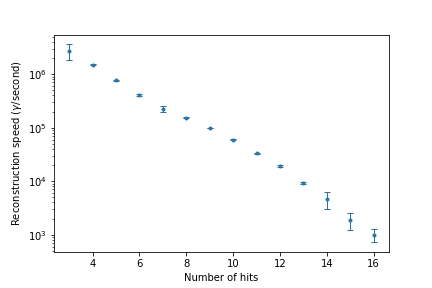
\includegraphics[width=0.7\textwidth]{graphs/pi_hits_speed.png}
    \caption{Caption}
    \label{fig:hits_speed}
\end{figure}

\begin{figure}
    \centering
    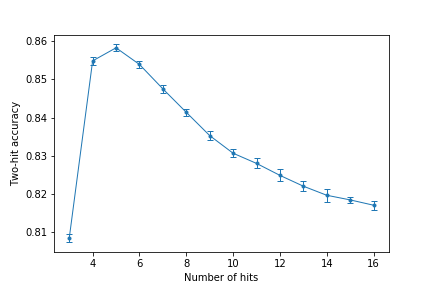
\includegraphics[width=0.7\textwidth]{graphs/pi_hits_acc.png}
    \caption{Caption}
    \label{fig:hits_acc}
\end{figure}

%%% Hits v hits Used

\section{Hits used in reconstruction}
- Accuracy seems to tail off around 6-8 hits for the toy model
- photons/sec goes down pretty linearly as we increase hits used
- We will likely see similar trends with Geant/real data, meaning we can fix a maximum number of hits to use (say, 10), and only sacrifice a few percentage points in accuracy while saving a significant amount of time on events with more hits.
- We expect that events with high numbers of hits will be much less likely than events with low numbers of hits, so there may be different optimal cutoffs for different source distributions.
- *** needs to be run again on the pi

\begin{figure}
    \centering
    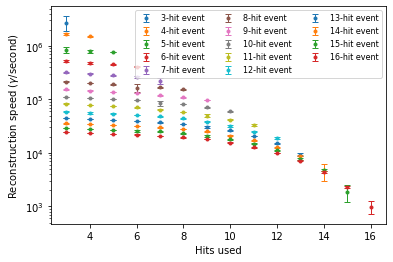
\includegraphics[width=0.7\textwidth]{graphs/pi_hits_v_hitsUsed_speed.png}
    \caption{Decrease in throughput with hits used in reconstruction}
    \label{fig:hits_v_hitsUsed}
\end{figure}

\begin{figure}
    \centering
    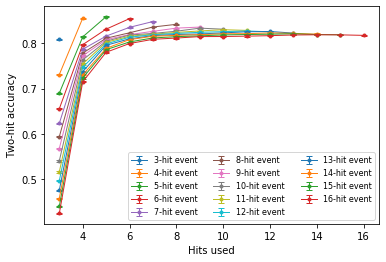
\includegraphics[width=0.7\textwidth]{graphs/pi_hits_v_hitsUsed_accuracy.png}
    \caption{Caption}
    \label{fig:my_label}
\end{figure}

\begin{figure}
    \centering
    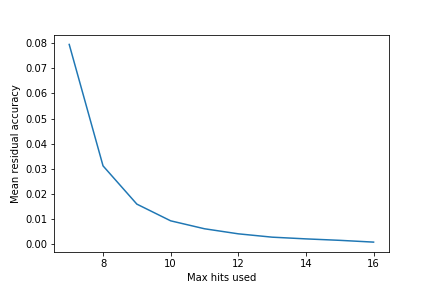
\includegraphics[width=0.7\textwidth]{graphs/mean_resid_acc.png}
    \caption{Caption}
    \label{fig:my_label}
\end{figure}

\section{p-value}
- visible correlation, but try to get a better one
- distinct downward trend in accuracy as p-value gets larger. This indicates we should use our highest p-value tested, and perhaps investigate even smaller ones.
- no clear trend in speed graph. Slight upward line until large error bar on 0.10 p-value

\begin{figure}
    \centering
    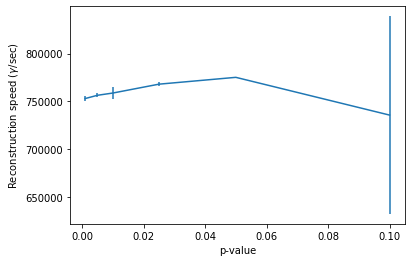
\includegraphics[width=0.7\textwidth]{graphs/pi_p_speed.png}
    \caption{Caption}
    \label{fig:my_label}
\end{figure}

\begin{figure}
    \centering
    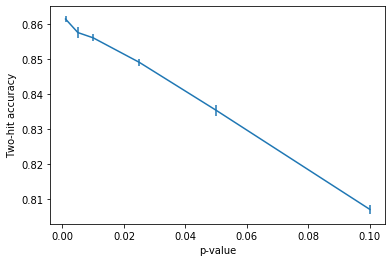
\includegraphics[width=0.7\textwidth]{graphs/pi_p_acc.png}
    \caption{Caption}
    \label{fig:my_label}
\end{figure}

\section{$\eta$-tolerance}
- There seems to be a slight periodic trend in the eta accuracy, though it is difficult to tell with the error bars
- could run with larger number of photons to find out for sure

\begin{figure}
    \centering
    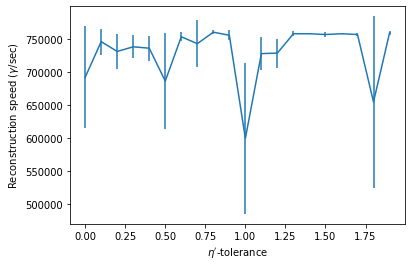
\includegraphics[width=0.7\textwidth]{graphs/pi_eta_speed.png}
    \caption{Caption}
    \label{fig:my_label}
\end{figure}

\begin{figure}
    \centering
    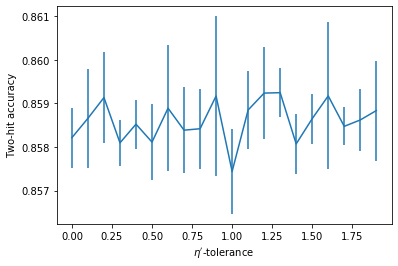
\includegraphics[width=0.7\textwidth]{graphs/pi_eta_acc.png}
    \caption{Caption}
    \label{fig:my_label}
\end{figure}

\section{Predicted Noise}
- speed for estimated energy noise has a slight downward trend, but the noise threshold is too high to draw any real conclusions. Most throughput values appear within a margin of about 10\%  of the assumed trend line.
- accuracy goes up by quite a bit when we predict more energy noise rather than less, but tails off at about 0.22, which is what the actual value of noise is. This could be incredibly useful in real-world applications, as we would be able to tell how much actual energy noise there is simply from a graph like this.
- of course, real-world applications are always more complicated, so this bears further research, but it is a promising indication.
- spatial noise does not allow us to draw many conclusions, as the ranges are so small that the error bars eclipse any minute trends in the data. 

\begin{figure}
    \centering
    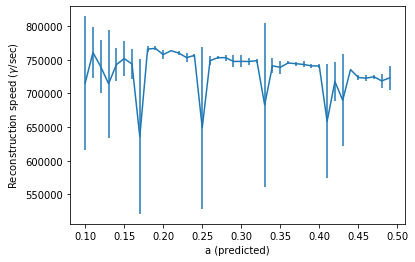
\includegraphics[width=0.7\textwidth]{graphs/pi_enFactor_speed.png}
    \caption{Caption}
    \label{fig:my_label}
\end{figure}

\begin{figure}
    \centering
    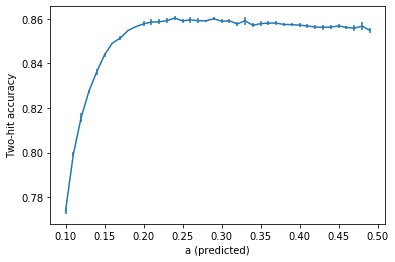
\includegraphics[width=0.7\textwidth]{graphs/pi_enFactor_acc.png}
    \caption{Caption}
    \label{fig:my_label}
\end{figure}

\begin{figure}
    \centering
    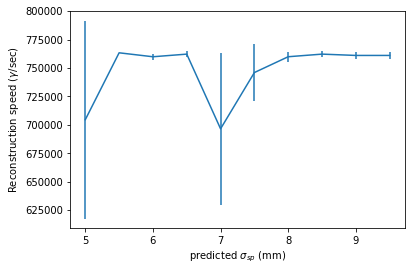
\includegraphics[width=0.7\textwidth]{graphs/pi_spFactor_speed.png}
    \caption{Caption}
    \label{fig:my_label}
\end{figure}

\begin{figure}
    \centering
    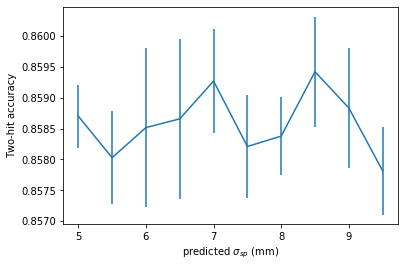
\includegraphics[width=0.7\textwidth]{graphs/pi_spFactor_acc.png}
    \caption{Caption}
    \label{fig:my_label}
\end{figure}

\section{Simulated Noise}
- helps with proof of concept - we want to check the trends are as we expect
- we expect accuracy to go down with increased noise, and it does for both
- we expect throughput to remain about the same, which it also does within some margin of error

\begin{figure}
    \centering
    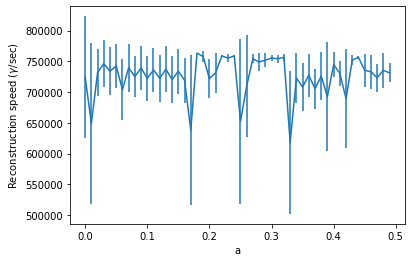
\includegraphics[width=0.7\textwidth]{graphs/pi_enNoise_speed.png}
    \caption{Caption}
    \label{fig:my_label}
\end{figure}

\begin{figure}
    \centering
    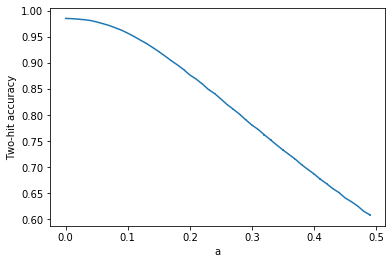
\includegraphics[width=0.7\textwidth]{graphs/pi_enNoise_acc.png}
    \caption{Caption}
    \label{fig:my_label}
\end{figure}

\begin{figure}
    \centering
    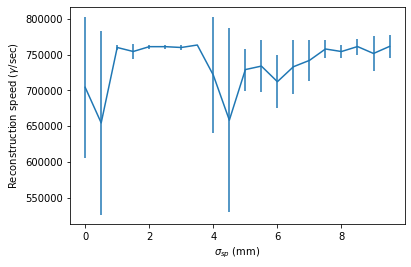
\includegraphics[width=0.7\textwidth]{graphs/pi_spNoise_speed.png}
    \caption{Caption}
    \label{fig:my_label}
\end{figure}

\begin{figure}
    \centering
    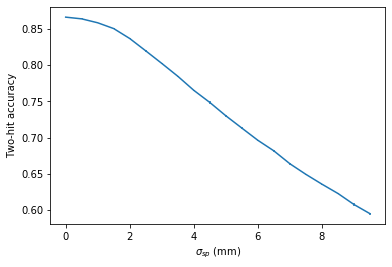
\includegraphics[width=0.7\textwidth]{graphs/pi_spNoise_acc.png}
    \caption{Caption}
    \label{fig:my_label}
\end{figure}

